% 2014-11-12
% DM1602 Materials Report

\documentclass[12pt,twocolumn, a4paper, titlepage]{article}
\usepackage[top=2.8cm, bottom=2.8cm, left = 2cm, right=2cm]{geometry}
\usepackage{fancyhdr}
\usepackage{blindtext}
\usepackage[none]{hyphenat}
\usepackage[hidelinks]{hyperref}
\usepackage{amssymb} % Symbols
\usepackage{chemfig}
\usepackage{graphicx}

\usepackage{siunitx} % Units
\sisetup{per-mode=symbol} % Sort out \per

% Biblatex settings - http://tex.stackexchange.com/questions/134258/harvard-style-bibliography-with-biblatex-almost-but-not-quite
\usepackage[
backend=biber,
useprefix=true,
maxcitenames=3,
maxbibnames=99,
style=authoryear,
dashed=false,
hyperref=true,
url=false
]{biblatex}

% Harvard Reference System stuff:
\DeclareNameAlias{author}{last-first}
\renewcommand*{\mkbibnamefirst}[1]{{\let~\,#1}} % insert thin spaces between author initials
\renewcommand*{\nameyeardelim}{\addcomma\addspace} % insert a comma between author and year in-text citations
\renewcommand*{\newunitpunct}{\addcomma\addspace} % comma as separator in bibliography, not full stop
\setlength\bibitemsep{1.5\itemsep} % increase spacing between entries in bibliography
\renewbibmacro{in:}{} % remove 'in:' preceding article title
\renewcommand*{\bibinitdelim}{} % Space between author initials

% Place volume number within parentheses:
\renewbibmacro*{volume+number+eid}{
    \printfield{volume}
    \setunit*{\addnbspace}% NEW (optional); there's also \addnbthinspace
    \printfield{number}
    \setunit{\addcomma\space}
    \printfield{eid}}
\DeclareFieldFormat[article]{number}{\mkbibparens{#1}}

% No punctuation after date in reference
\usepackage{xpatch}\xapptobibmacro{date+extrayear}{\nopunct}{}{}

% If online resource, show url
\AtEveryBibitem{%
    \ifentrytype{online}{%
    }{%
        \clearfield{url}%
        \clearfield{urldate}%
    }%
}


% Use \cite for referencing name and \pcite for author-year
\let\cite\textcite
\let\pcite\parencite
\addbibresource{refs.bib}

% Stop right-justifying section headings
\usepackage{sectsty}
\allsectionsfont{\raggedright}

% Make sections start a new page
%\let\stdsection\section
%\renewcommand\section{\newpage\stdsection}

\graphicspath{images/}

\begin{document}
\begin{titlepage}
\begin{flushright}
\null
\vfill
\rule{16cm}{1.5pt}\\[3mm]
\textsc{\Huge Materials for hammock suspension}\\
\textsc{\Large DM1602 Materials report}\\
\rule{16cm}{1pt}\\[3mm]
\vspace{8cm}
\rule{3.5cm}{1pt}\\
\textsc{\large George Bryant}\\
\#1418415
\end{flushright}
\end{titlepage}

\tableofcontents

\clearpage
\section{Workshop Experience}
So far in this module I have completed the wood and plastics workshops. Both have been useful experiences and I have learned a lot about working quickly making best use of the power tools available, having in the past mostly used hand tools.

In the wood workshop I gained some valuable experience with different woods. Working with the pine with hand tools was similar to the woodwork I was used to. The loose grain of the wood meant that it chipped or tore easily when going the wrong direction along the wood's grain, as the grain usually did not perfectly align with the edge of the piece.

The plastics workshop was more of a new experience; I had worked with acrylic before, but never with multiple sheets glued together. It proved to be a very different experience to what I expected. Acrylic has a low toughness, and in the past my tools had evidently not been sharp enough to cut it, meaning it cracked easily and frequently. With properly maintained tools, and especially with multiple layers laminated together, the acrylic becomes much easier to work with.

While the plastics workshop deals only with acrylic, I wanted to research some other polymers, and I needed a context to relate them to. Something I have been very enthusiastic about in the past is hammock camping. When a hammock is tied between two trees it can put the rope in very high tension, which requires materials with a certain set of properties. I decided to investigate these properties and the materials which we use for ropes.

\section{Mechanics of hammock suspension}
\label{sec:mechanics}
I will attempt to keep the mechanics brief as this report is intended to focus on the materials side of hammock suspension. Forces involved in hammock suspension are much larger than one would expect. This is due to the angles involved. If we simplify a hammock to a model consisting of two ropes holding up a weight (Figure \ref{fig:hammock}), we can calculate a rough value for the tension in the ropes.

\begin{figure}
\centering
\begin{tikzpicture}
\coordinate[](T1) at (0,3);
\coordinate[](T2) at (6,3);
\coordinate[](W) at (3,0);
\coordinate[](C) at (3,2);
\coordinate[](H_start) at (4,3);
\coordinate[](H_end) at (7,3);

% Draw force arrows
\draw [thick,->] (C) -- (T1) node[anchor=north, yshift=-0.15cm] {$T_1$};
\draw [thick,->] (C) -- (T2) node[anchor=north, yshift=-0.15cm] {$T_2$};
\draw [thick,->] (C) -- (W) node[anchor=west] {$W$};
\draw [thick, dashed] (H_start) -- (H_end);

% Draw arc
\draw (4,3) arc (180:216.8:1cm) node[midway, left] {$\theta$};

\end{tikzpicture}
\caption{Simplified diagram of hammock}
\label{fig:hammock}
\end{figure}

Weight W is opposed by the y-components of the two rope tensions, such that each $T_y = 0.5W$. Naming the angle between the rope and the horizontal $\theta$, we can see that:
$$\sin\theta = \frac{T_y}{T}$$
$$\therefore T = \frac{T_y}{\sin\theta} = \frac{0.5 \times W}{\sin\theta}$$

Assuming an average British male weight of \SI{83.6}{\kilogram} \pcite{ons_average_2010} and a hang angle of \ang{30} -- the recommended angle for comfort in a hammock \pcite{dream_hang} -- we can calculate the tension in the ropes.
$$T = \frac{0.5 \times 83.6 \times 9.81}{\sin30}$$
$$\therefore T = \SI{820}{\newton}$$
This seems a fairly reasonable load, but it quickly grows greater as the angle $\theta$ decreases---reaching \SI{2360}{\newton} at only \ang{10}. This could present a problem to the rope if the hammock is hung improperly, and is especially the case when presented with the dynamic loading caused by jumping or falling into the hammock.

With a \SI{5}{\milli\metre} diameter rope of cross-sectional area \SI{19.6}{\milli\metre\squared}, this means a stress of $\SI{2360}{\newton} \div \SI{1.96e-5}{\metre\squared} = \SI{120}{\mega\pascal}$.
%\subsection{Knots and splices}



\section{Ropes used for hammock suspension}
\subsection{Nylon and polyester webbing}
A common material for hammock suspension is fabric strips woven from nylon or polyester, known as webbing. It is used mainly because it is cheap, readily available and due to its width (\SIrange{25}{50}{\milli\metre}), which means it is unlikely to damage trees.

One problem that webbing exhibits is stretching when weight is applied. This stretching is greater in nylon webbing---20-30\% as opposed to polyester's 15-25\% \pcite{tie_down_faq}, so polyester webbing is more often used. This stretch can result in a sub-optimal ''hang`` for the camper, as the strap length increases overnight.

A fairly typical price for \SI{25}{\milli\metre} polyester webbing is £0.50 per metre. This makes it very cheap for hammock campers to buy, and its \SI{1500}{\kilo\gram} breaking strength \pcite{25mm_poly_webbing} means it is more than strong enough to withstand normal usage. At \SI{25}{\milli\metre} wide and \SI{1.25}{\milli\metre} thick, a \SI{1500}{\kilo\gram} mass would apply a strain of $1500 \times 9.81 \div (\num{25e-3} \times \num{1.25e-3}) = \SI{470}{\mega\pascal}$. This is far higher than the expected strains calculated in section \ref{sec:mechanics}, so this webbing is far stronger than needed for hammock suspension.

\subsection{High modulus polyethylene ropes}
However, such webbing is bulky, making it difficult to carry when hiking. A more lightweight, smaller alternative is needed for some campers. They usually turn to high-modulus polyethylene ropes, marketed as Dyneema or Spectra, which also solve the problem of stretching.

Ultra-high molecular weight polyethylene is the main material I will investigate in this report. Higher priced but stronger than nylon webbing, woven polyethylene ropes tend to be marketed at sailing enthusiasts rather than as general purpose cords. They are prized among those who use them for their low weight, low bulk and high strength.

\section{High modulus polyethylene}
High modulus polyethylene (HMPE) or ultra-high-molecular-weight polyethylene (UHMWPE) is so called because it consists of very long chains of polyethylene. Having a longer chain length than other forms of polyethylene, HMPE has more interaction between different chains, and thus has a higher stiffness, despite the low strength of the individual van der Waals bonds.

\subsection{Production}
Initially, long polyethylene fibres (``macrofibrillar crystals'') were produced from a solution of linear polyethylene (figure \ref{fig:pe}), which is mostly linear with only short branches, in p-xylene (figure \ref{fig:p-xylene}). A long crystal was grown from the side of a rotating cylinder containing the solution (figure \ref{fig:grow_pe}). This produced fibres which reduced in diameter as they grew, and so were not particularly useful \pcite{zwijnenburg_longitudinal_1976}.

\newcommand\setpolymerdelim[2]{\def\delimleft{#1}\def\delimright{#2}}
\def\makebraces[#1,#2]#3#4#5{%
\edef\delimhalfdim{\the\dimexpr(#1+#2)/2}%
\edef\delimvshift{\the\dimexpr(#1-#2)/2}%
\chemmove{%
\node[at=(#4),yshift=(\delimvshift)]
{$\left\delimleft\vrule height\delimhalfdim depth\delimhalfdim
width0pt\right.$};%
\node[at=(#5),yshift=(\delimvshift)]
{$\left.\vrule height\delimhalfdim depth\delimhalfdim
width0pt\right\delimright_{\rlap{$\scriptstyle#3$}}$};}}
\setpolymerdelim()
\begin{figure}
\centering
\chemfig{\vphantom{CH_2}-[@{op,.75}]CH_2-CH_2-[@{cl,0.25}]}
\makebraces[5pt,5pt]{\!\!n}{op}{cl}
\caption{Polyethylene's repeating unit}
\label{fig:pe}
\end{figure}

\begin{figure}
\centering
\chemfig{H_3C-*6(-=-(-CH_3)=-=)}
\caption{p-xylene molecule}
\label{fig:p-xylene}
\end{figure}

\begin{figure}
\centering
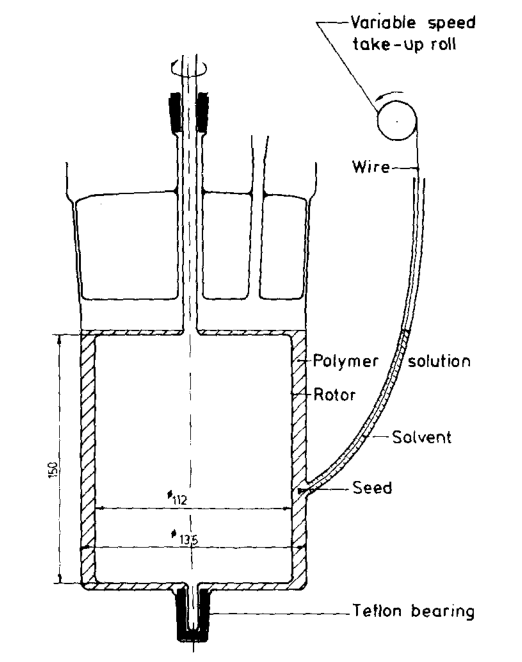
\includegraphics[width=0.8\columnwidth]{images/growing_polyethylene}
\caption{Growing polyethylene fibres using a Couette instrument \pcite{zwijnenburg_longitudinal_1976}}
\label{fig:grow_pe}
\end{figure}

A more easily commercialised method of production is the spinning and drawing of polyethylene filaments. The solution containing polyethylene is extruded through small nozzles in a spinneret \pcite{polymer_spinning}, producing a polyethylene fibre, and this goes through a cooling bath and then an oven at \SI{120}{\celsius}---below the melting point of the polymer.

While in the oven, in the method of \cite{smith_ultra-high-strength_1980} the fibres are stretched at a strain rate of around \SI{1}{\per\second}, which aligns the polyethylene chains. Smith and Lemstra explain that the fibre is stretched after being cooled because it reduces the relaxation effect---in the liquid state macromolecules exhibit a ``relatively rapid relaxation''. The oven drawing has the added benefit of evaporating all detectable quantities of the solvent from the fibres, leaving only polyethylene.

\subsection{Properties}
This method produces polyethylene fibres with a tensile strength and modulus dependent on the draw ratio. The draw ratio is the ratio of the cross-sectional area of the un-drawn fibres to that of the drawn ones.

As you can see from figure \ref{fig:pe_fibre_ss}, as the polymer is drawn out more, the ultimate tensile strength increases, up to \SI{3.04}{\giga\pascal} at a ratio of $31.7$. This shows that the increased crystallinity caused by drawing the fibres does have a positive effect on the tensile strength.

The modulus of Smith and Lemstra's most highly drawn polyethylene is \SI{90.2}{\giga\pascal}, around half that of steel. The fibre makes up for its lower stiffness with a much higher tensile strength than steel.

\begin{figure}
\centering
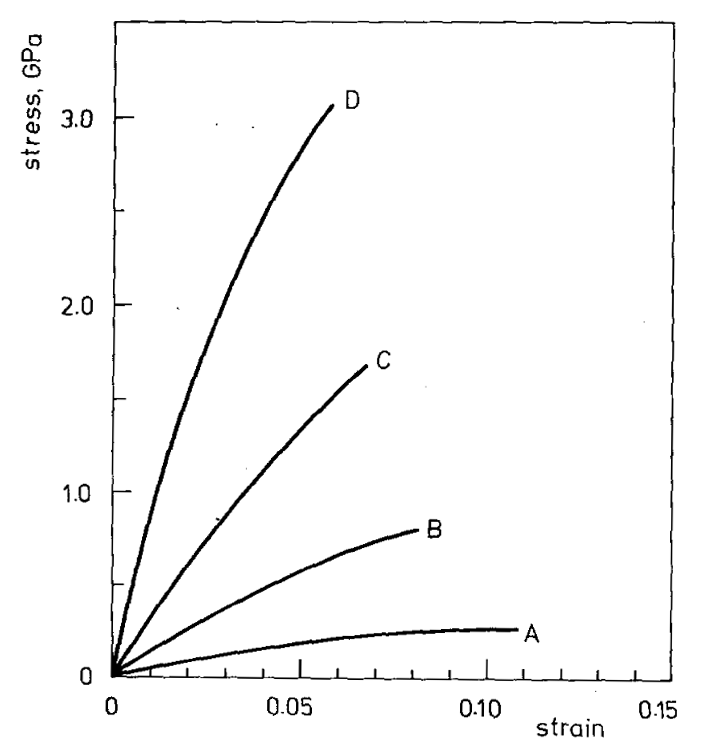
\includegraphics[width=0.8\columnwidth]{images/pe_stress_strain}
\caption{Stress-strain curves of polyethylene fibres. Draw ratios: A 2.8; B 8.4; C 15.7; D 31.7 \pcite{smith_ultra-high-strength_1980}}
\label{fig:pe_fibre_ss}
\end{figure}

\subsubsection{Effects of crosslinking}
Another application for which UHMWPE is used is  human joint replacement, in which the polymer acts as a synthetic cartilage. In the lower part of the knee joint, the polymer "undergoes cyclic stresses as high as \SIrange{10}{15}{\mega\pascal} in tension and \SIrange{30}{40}{\mega\pascal} in compression" \pcite{simis_combined_2006}. Simis et.\ al.\ explore the effects of crosslinking on the microstructural and mechanical properties of UHMWPE.

The extra crosslinks were created by subjecting samples of the polymer to ionising radiation. The source used was a \SI{5}{\kilo\gray} gamma ray source. The samples were then held above their melting temperature at \SI{170}{\celsius} for \SI{4}{\hour} "to complete the crosslinking and annihilate free radicals" \pcite{simis_combined_2006}. High pressure variants were created by subjecting the polyethylene to pressures of \SI{500}{\mega\pascal} shortly before cooling.

All specimens had a layered appearance in their microstructure, but that of the irradiated specimens had a much smaller lamellae thickness. This was especially apparent in the high pressure variant, where the thickness was \SI{50.6}{\nano\metre} compared to the non-irradiated specimen's \SI{131.2}{\nano\metre}.

The effect this has on the properties is unexpected. The tensile modulus is decreased in the low-pressure variants, and there is only a statistically insignificant increase in the high pressure variant. What this means is that the increased cross-linking does not have a positive effect on the modulus.

The ultimate tensile strength, however, is (at least for the high pressure samples) increased from \SI{78.8}{\mega\pascal} to \SI{167.8}{\mega\pascal}. The low-pressure variants show an equally significant decrease in tensile strength.

\cite{muratoglu_unified_1999} note that while a number of mechanical properties are decreased by the increased crosslinking, the wear resistance does increase, which was the aim of the original experiments by \cite{simis_combined_2006}

What this means is that while the radiation-induced crosslinking has produced an interesting effect on the microstructure of the polymer, it has not had an effect which would be useful for hammock suspension.

\subsection{How the properties are useful}

\newpage\section{Conclusion}
% Relate back to hammock ropes
% Talk about how future advances could help properties

\clearpage
\printbibliography[heading=bibintoc]
\end{document}